\section{Stationary Current Distribution}

Since $\frac{\partial}{\partial t} = 0$ the Continuity Equation can be written as

\begin{tabular}{ll}
	\(\displaystyle \nabla \cdot \vec{J} = -\frac{\partial \rho}{\partial t} =  0\) \\
	\(\displaystyle \nabla \cdot \vec{J} = 0 \rightarrow \nabla \cdot \left(\sigma \vec{E}\right) \rightarrow \nabla \cdot \left(\sigma V \varphi\right) = 0\) \\
\end{tabular}

Thus, the PDE is
\begin{equation*}
	\frac{\partial}{\partial x}\left(\sigma \frac{\partial \varphi}{\partial x}\right) +\frac{\partial}{\partial y}\left(\sigma \frac{\partial \varphi}{\partial y}\right)
	+\frac{\partial}{\partial z}\left(\sigma \frac{\partial \varphi}{\partial z}\right) = 0, \left(x,y,z\right) \in \Omega \subseteq R^2
\end{equation*}

\textbf{\\ Boundary Value Problem (BVP)\\}
\begin{minipage}[lt]{11cm}
	\begin{tabular}{l}
		\(\displaystyle \frac{\partial}{\partial x}\left(\sigma \frac{\partial V}{\partial x}\right) +\frac{\partial}{\partial y}\left(\sigma \frac{\partial V}{\partial y}\right)
		= 0, \left(x,y\right) \in \Omega \subseteq R^2 \) \\ \\
		\(\displaystyle \frac{\partial V}{\partial n} = 0, \left(x,y\right) \in \partial_{N1} \Omega\) \\
		\(\displaystyle \frac{\partial V}{\partial n} = \frac{I}{\sigma \cdot S_{N2}}, \left(x,y\right) \in \partial_{N2} \Omega\) \\
		\(\displaystyle V\left(x,y\right) = 0, \left(x,y\right) \in \partial_D \Omega\)\\ \\
		
		\(\displaystyle \partial_D\Omega\cup\partial_{N1}\Omega\cup\partial_{N2}\Omega = \partial\Omega = \text{boundary}(\Omega) \)\\
		\textbf{One BC must be a Dirichlet-BC!}
	\end{tabular}
\end{minipage}
\begin{minipage}[rt]{8cm}
	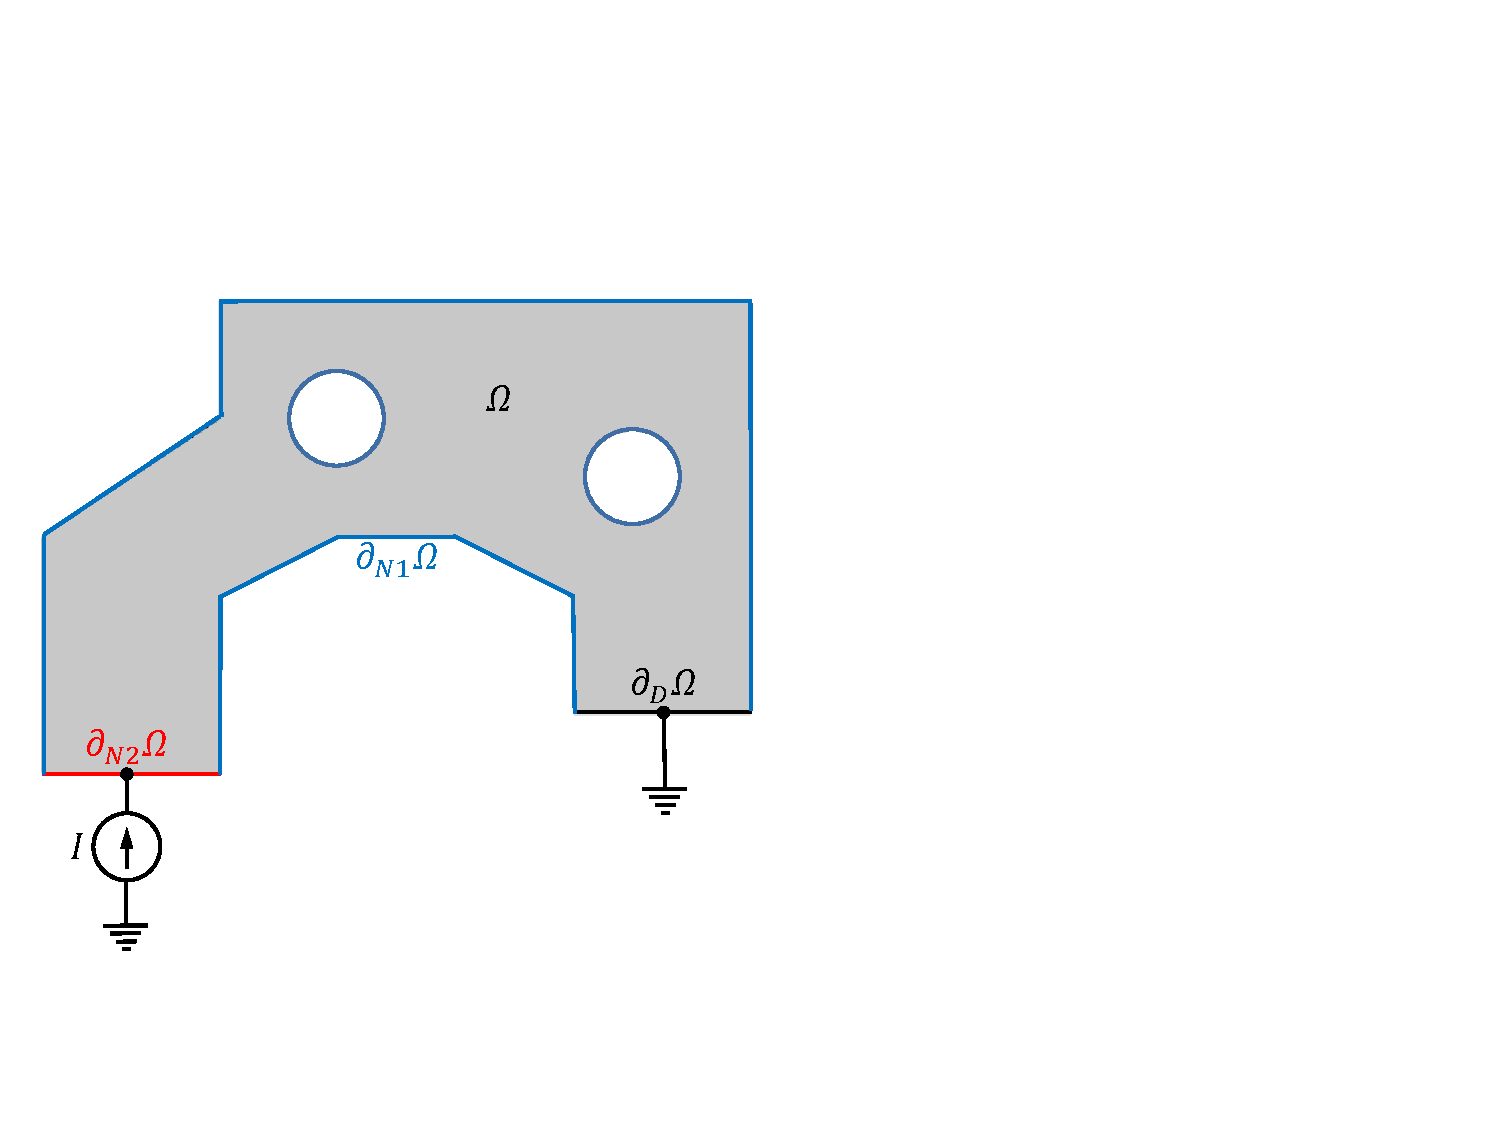
\includegraphics[width=.8\textwidth]{./images/CurrentDistribution.pdf}
\end{minipage}

\textbf{\\ \\ Post processing \\ }
\begin{tabular}{ll}
	Loss density $\left[\frac{W}{m^3}\right]$: & \(\displaystyle p_L = \vec{J} \cdot \vec{E} = \sigma \cdot \vec{E}^2 = \frac{\vec{J}^2}{\sigma} \)\\
	Total losses $[W]$: & \(\displaystyle P_L = \iiint\limits_{\left(V\right)} p_L \cdot dV = \iiint\limits_{\left(V\right)} \sigma \cdot \vec{E}^2 \cdot dV \) \\
	Resistance $[\Omega]$: & \(\displaystyle R = \frac{P_L}{I^2}\) \\
\end{tabular}